\section{Results}\label{sec:results}

\subsection{Pipeline statistics}\label{sec:selection}
\Cref{tab:stages} traces the exposures through the pipeline. All \NDayside{} dayside exposures with valid geometry were fitted; no flux-percentile pre-selection was applied. \NMapped{} spectra (\PctMapped\% of the dayside set) pass every quality criterion and form the mapping set. The fraction passing varies strongly with solar activity. It ranges from \PassMinPct\% in \PassMinMonth{}, near solar minimum, where most spectra fall below the count threshold or below GOES B1, to \PassMaxPct\% in \PassMaxMonth{}, with a median of \PassMedPct\% over the \NMonths{} months (\cref{tab:months}). The GOES temperatures of the mapped exposures have a median of \MapTmed{}\,MK (5th--95th percentile \MapTlo--\MapThi{}\,MK).

\begin{table}[t]
\centering
\caption{Exposure counts (all 24 months). The indented rows are independent subsets of the dayside set, not sequential stages; the mapping set satisfies all criteria at once.}\label{tab:stages}
\small
\begin{tabular}{lr}
\toprule
Stage & Exposures \\
\midrule
Level-1 files & \NRawFiles \\
Dayside, valid geometry (all fitted) & \NDayside \\
\quad of which: reliable GOES temperature ($\geq$ B1) & \NGoesOK \\
\quad of which: fit converged & \NConverged \\
Mapping set (all quality criteria, \cref{sec:uncert}) & \NMapped \\
\bottomrule
\end{tabular}
\end{table}

\subsection{Fit examples}\label{sec:examples}
\Cref{fig:fits} shows fits to a bright, a median and a faint dayside spectrum. The model describes the Mg, Al and Si K lines, the Ca K line and the scattered solar continuum and lines. In the faint spectrum the particle background dominates above \SI{2}{keV}, and the uncertainties on Mg/Si and Al/Si become correspondingly large.  Bright flare spectra (e.g.\ panel (a), $T=16.8$\,MK) often fail the goodness-of-fit criterion. Residual structure below \SI{2}{keV} points to limitations of the isothermal solar spectrum and of the line-shape model, so the mapping set is weighted towards non-flaring and moderate-flare conditions.

\begin{figure*}[!tp]
\centering
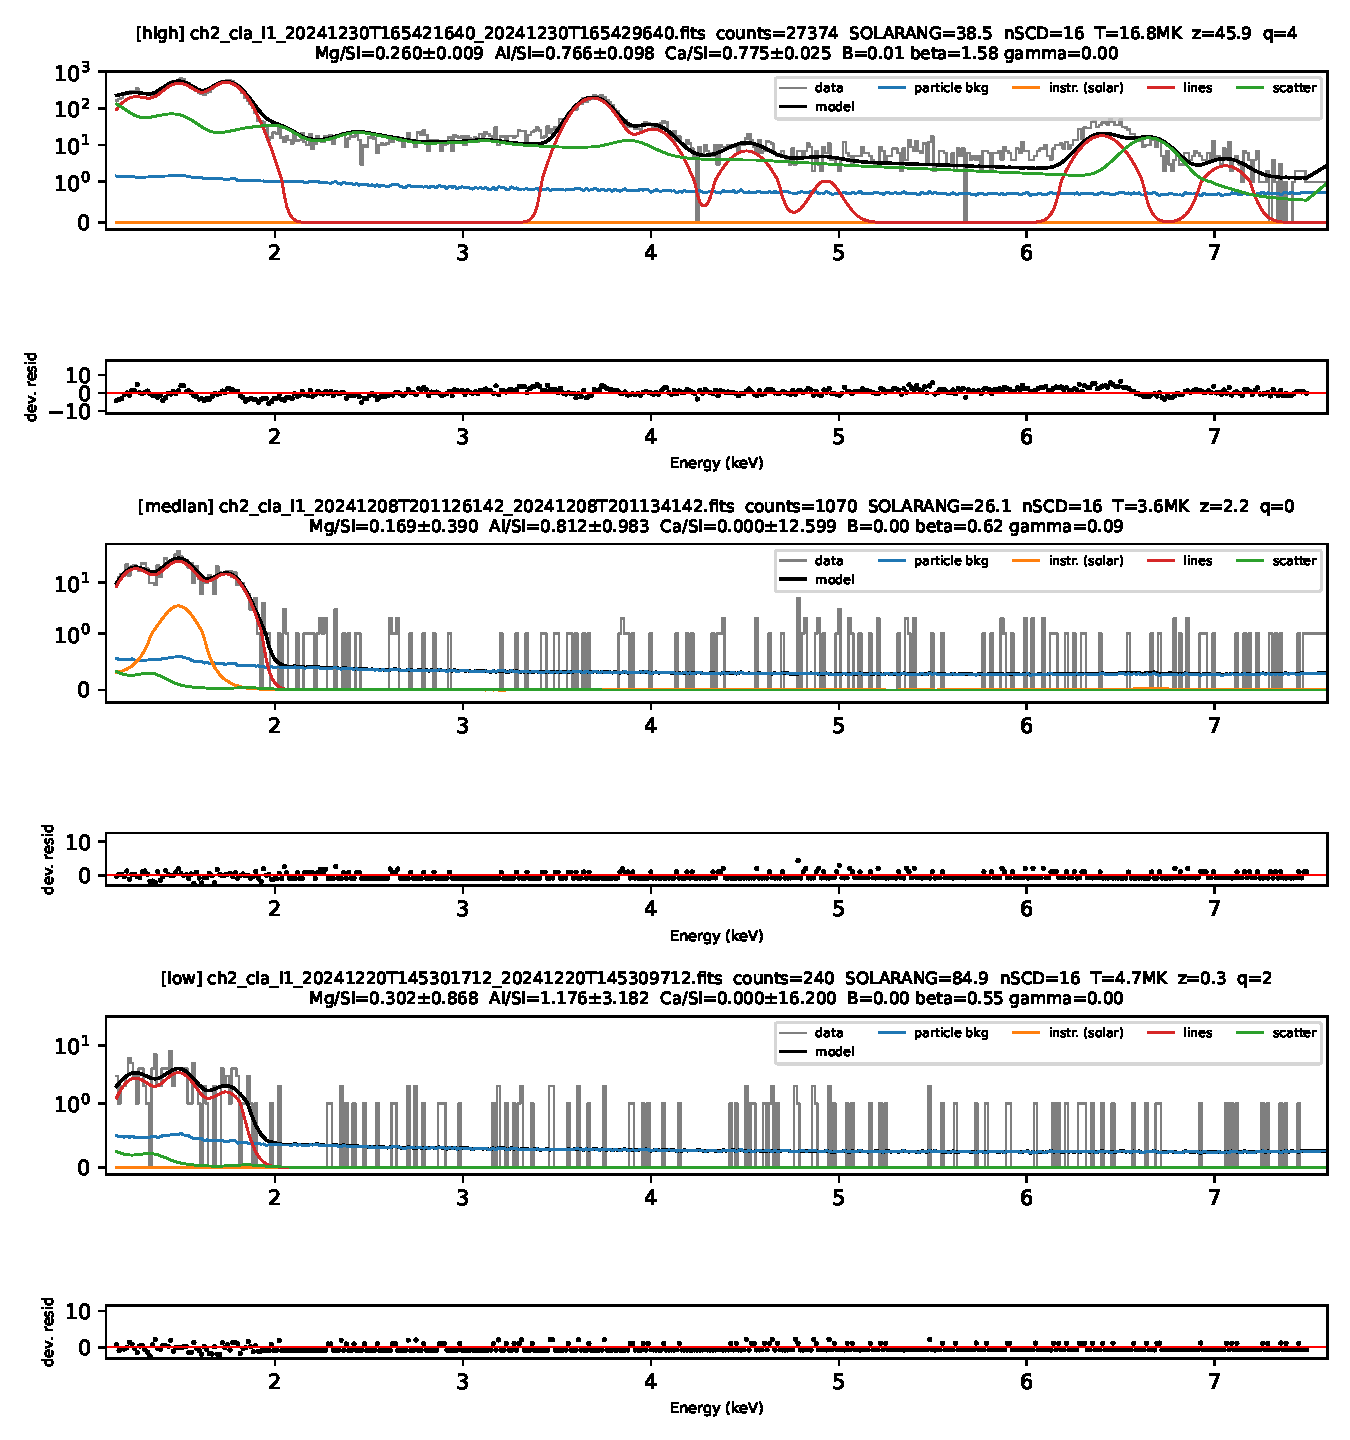
\includegraphics[width=\textwidth]{figures/fig_fits.pdf}
\caption{Example spectral fits. Fits to (a) a bright, (b) a median and (c) a faint dayside spectrum from December 2024: data (grey steps), total model (black), fluorescence lines (orange, solid), scattered solar spectrum (purple, dotted) and particle background (blue, dashed), each with deviance residuals below. The annotation in each panel gives the counts in the fitted window, the GOES temperature, the goodness-of-fit $z$ and the fitted Mg/Si and Al/Si with their $1\sigma$ uncertainties.}\label{fig:fits}
\end{figure*}

\subsection{Global maps}\label{sec:maps}
\Cref{fig:maps} shows the Mg/Si and Al/Si maps with their observation-count and standard-error layers. Over the mapping set, the median footprint ratios are Mg/Si $=\MedMg$ (5th--95th percentile \PfiveMg--\PninetyfiveMg) and Al/Si $=\MedAl$ (\PfiveAl--\PninetyfiveAl). The Mg/Si range lies within the range of returned lunar soils. The Al/Si median is higher than most returned soils, which may indicate a residual efficiency or calibration offset between the Al and Si lines (\cref{sec:limitations}). An offset of this kind would scale all values without changing the spatial pattern or the correlations, so we regard the maps as relative.

Quality-0 footprints reach every 2\textdegree{} cell (\CovUsedCells\% of cells, \CovUsedArea\% of the area), and \CovFiveArea\% of the surface is covered by cells with at least five footprints. The coverage comes from the polar orbits of the 24 archives at all local times, not from interpolation. The polar cells have the fewest footprints and the largest standard errors.

The Mg/Si map shows the expected first-order dichotomy: higher values over the nearside maria and the South Pole--Aitken basin, lower values over the farside feldspathic highlands. The Al/Si map shows the complementary pattern at higher contrast. Several maria (Imbrium, Serenitatis, Crisium, Tranquillitatis, Fecunditatis, Nubium, Humorum) and the South Pole--Aitken basin appear as low-Al/Si units against the feldspathic highlands. Residual north--south striping follows individual orbits. We attribute it mainly to orbit-to-orbit differences in the solar state that the GOES isothermal temperature does not fully capture (\cref{sec:discussion}).

\begin{figure*}[!tp]
\centering
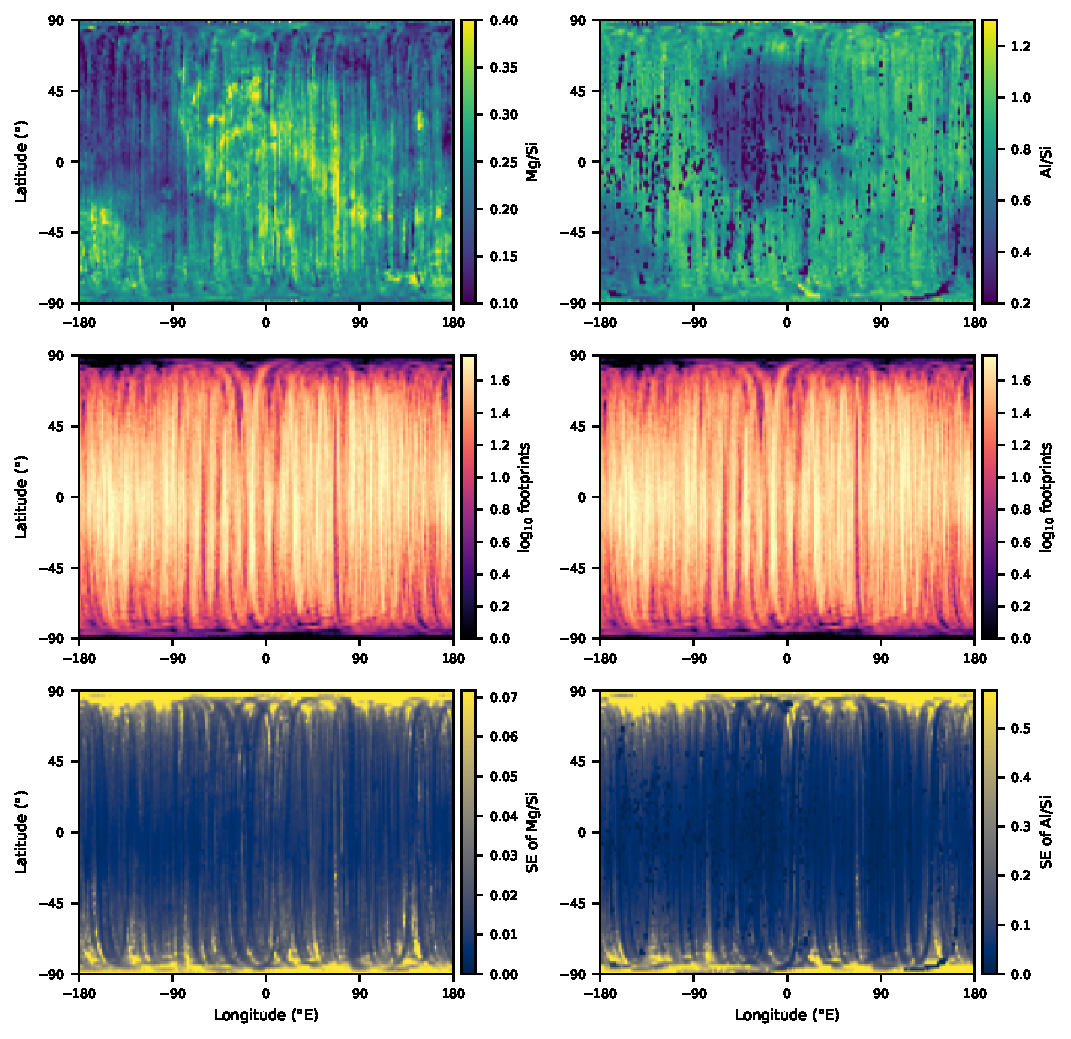
\includegraphics[width=\textwidth]{figures/fig_maps.pdf}
\caption{Global Mg/Si and Al/Si maps with quality layers. Mg/Si (left) and Al/Si (right) weight ratios on a 2\textdegree{} grid (inverse-variance-weighted means of quality-0 footprints; no smoothing or infill), with the number of footprints per cell (middle) and the standard error of the cell mean (bottom).}\label{fig:maps}
\end{figure*}
